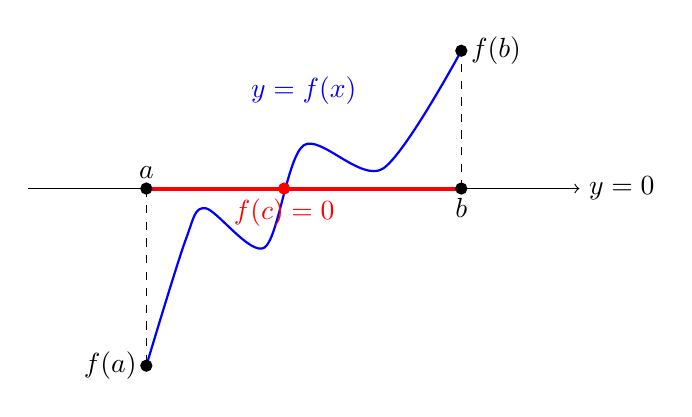
\begin{tikzpicture}[scale=1,domain=0:6]
	% Draw the axes
	\draw[->] (-0.5,-1.75) -- (6.5,-1.75) node[right] {$y=0$};
%	\draw[->] (0,-4.5) -- (0,0) node[above] {$y$};
	
	% Define points a and b on the x-axis
	\coordinate (A) at (1,-1.75);
	\coordinate (B) at (5,-1.75);
	
	% Define points f(a), f(b) and gamma
	\coordinate (FA) at (1,-4); % f(a)
	\coordinate (FB) at (5,0); % f(b)
	\coordinate (GAMMA) at (0,2.5); % gamma horizontal line
	
	% Function graph
	\draw[color=blue,thick,smooth] plot coordinates {(1,-4) (1.5,-2.4) (1.75,-2) (2.5,-2.5) (3,-1.2) (4,-1.5) (5,0)};
	\node[blue] at (3,-.5) {$y=f(x)$};
	
	% Points on the graph
	\filldraw[black] (FA) circle (2pt) node[left] {$f(a)$};
	\filldraw[black] (FB) circle (2pt) node[right] {$f(b)$};
	
	% Draw vertical dashed lines for a and b
	\draw[dashed] (A) -- (FA);
	\draw[dashed] (B) -- (FB);
	
	% Labels for a and b
	\node[above] at (A) {$a$};
	\node[below] at (B) {$b$};
	
	\draw[red, line width=.5mm] (A) -- (B);
	\filldraw[black] (1,-1.75) circle (2pt);
	\filldraw[black] (5,-1.75) circle (2pt);
	
	% Intersection point at c
	\filldraw[red] (2.75,-1.75) circle (2pt) node[below] {$f(c) = 0$};
\end{tikzpicture}
